\chapter{Otimização de Knuth-Yao}
\label{KY}

%----------------------------------------------------------------------------------------

O problema da árvore de busca binária ótima~\cite{CLRS} é um exemplo clássico de aplicação de programação dinâmica que é facilmente resolvido em tempo~$\Cl{O}(n^3)$, onde~$n$ é o número de chaves da árvore. Esta solução associa o custo de cada subárvore a uma entrada de uma matriz~${ n \times n }$ e relaciona tais entradas por meio de uma recorrência, reduzindo o problema original a resolver a recorrência. Aproveitando algumas propriedades não óbvias desta recorrência, Knuth~\cite{Knuth:1971} apresentou uma forma de resolvê-la em tempo~$\Cl{O}(n^2)$, o que agiliza a solução do problema original.

Mais tarde, a solução de Knuth foi estudada por Yao~\cite{Yao:1980,Yao:1982}, que mostrou que as propriedades observadas por Knuth eram consequência do fato de que a matriz em questão era Monge convexa. Desta maneira, foi possível perceber que a otimização de Knuth poderia ser útil em vários outros problemas de programação dinâmica. 

Bein, Golin, Larmore e Zhang~\cite{Bein:2009} buscaram enfraquecer a condição encontrada por Yao e mostraram que as matrizes derivadas dos problemas agilizados com a otimização de Knuth-Yao podem ser decompostas de três maneiras diferentes em matrizes totalmente monótonas. Com estas decomposições, é possível resolver ainda mais problemas. As descobertas do artigo citado neste parágrafo não serão discutidas aqui. Esta introdução foi baseada em tal artigo.

Vamos discutir os resultados observados por Yao, descrever a técnica desenvolvida por Knuth e aplicar este conhecimento para resolver um problema de programação dinâmica de forma mais eficiente do que a trivial.

%----------------------------------------------------------------------------------------

\section{Definições básicas} \label{KY:defs}

Vamos apresentar a otimização de Knuth-Yao para problemas de minimização, o que nos leva a trabalhar com convexidade. É fácil adaptar o conhecimento discutido neste capítulo para problemas de maximização, porém, em vez da convexidade, a concavidade deve ser usada para provar os resultados e modelar os problemas de interesse.

\begin{defi}[Recorrência de intervalos] \label{ KY:recint }
Uma matriz~$A \in \B{Q}^{n \times n}$ triangular inferior em 0 é considerada uma recorrência de intervalos se existe uma matriz~$C \in \B{Q}^{n \times n}$ tal que, para todo~$i,j \in [n]$,
\begin{equation*}
A[i][j] = \begin{cases}
C[i][j]                                                           & \text{se } i = j \text{, }  \\
C[i][j] + \min\{A[i][k-1] + A[k][j] \mid i < k \leq j \}          & \text{se } i < j \text{.}
\end{cases}
\end{equation*}
A matriz~$C$ é chamada de matriz de custos de~$A$.
\end{defi}

É fácil resolver uma recorrência desta forma em tempo~$\Cl{O}(n^3)$. Existe uma interpretação interessante deste tipo de recorrência que corresponde a vários problemas cuja a solução é baseada em programação dinâmica. Inicialmente, existe um vetor~$v \in \B{Q}^n$. É possível dividir este vetor em duas partes, isto é, escolher uma posição~$k \in [n-1]$ e substituir o vetor original pelos seus dois subvetores~$v[1 \tdots k]$ e~$v[k+1 \tdots n]$. Cada subvetor gerado pode ser dividido novamente. O custo de dividir um subvetor~$v[i \tdots j]$ qualquer de~$v$ é dado pela matriz~$C[i][j]$. O problema consiste em dividir um vetor original sucessivamente até transformá-lo em~$n$ vetores de tamanho unitário minimizando o custo de realizar todas as divisões.

\begin{figure}[h]
    \centering
    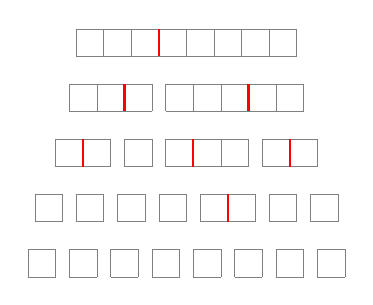
\begin{tikzpicture}[scale=.35]\footnotesize

\begin{scope}[yscale=-1] % I'm flipping the y-axis because I'm working on grids
  \pgfmathsetmacro{\p}{0} % initial y
  \draw[step=1cm,gray,very thin] (0,\p) grid (8,\p+1); % vector
  \draw[red,thick] (3,\p) -- (3,\p+1);

  \pgfmathsetmacro{\p}{2}
  \draw[xshift=-.25cm,step=1cm,gray,very thin] (0,\p) grid (3,\p+1);
  \draw[xshift=-.25cm,red,thick] (2,\p) -- (2,\p+1);
  \draw[xshift=.25cm,step=1cm,gray,very thin] (3,\p) grid (8,\p+1);
  \draw[xshift=.25cm,red,thick] (6,\p) -- (6,\p+1);

  \pgfmathsetmacro{\p}{4}
  \draw[xshift=-.75cm,step=1cm,gray,very thin] (0,\p) grid (2,\p+1);
  \draw[xshift=-.75cm,red,thick] (1,\p) -- (1,\p+1);
  \draw[xshift=-.25cm,step=1cm,gray,very thin] (2,\p) grid (3,\p+1);
  \draw[xshift=.25cm,step=1cm,gray,very thin] (3,\p) grid (6,\p+1);
  \draw[xshift=.25cm,red,thick] (4,\p) -- (4,\p+1);
  \draw[xshift=.75cm,step=1cm,gray,very thin] (6,\p) grid (8,\p+1);
  \draw[xshift=.75cm,red,thick] (7,\p) -- (7,\p+1);

  \pgfmathsetmacro{\p}{6}
  \draw[xshift=-1.5cm,step=1cm,gray,very thin] (0,\p) grid (1,\p+1);
  \draw[xshift=-1cm,step=1cm,gray,very thin] (1,\p) grid (2,\p+1);
  \draw[xshift=-.5cm,step=1cm,gray,very thin] (2,\p) grid (3,\p+1);
  \draw[xshift=0cm,step=1cm,gray,very thin] (3,\p) grid (4,\p+1);
  \draw[xshift=.5cm,step=1cm,gray,very thin] (4,\p) grid (6,\p+1);
  \draw[xshift=.5cm,red,thick] (5,\p) -- (5,\p+1);
  \draw[xshift=1cm,step=1cm,gray,very thin] (6,\p) grid (7,\p+1);
  \draw[xshift=1.5cm,step=1cm,gray,very thin] (7,\p) grid (8,\p+1);

  \pgfmathsetmacro{\p}{8}
  \draw[xshift=-1.75cm,step=1cm,gray,very thin] (0,\p) grid (1,\p+1);
  \draw[xshift=-1.25cm,step=1cm,gray,very thin] (1,\p) grid (2,\p+1);
  \draw[xshift=-.75cm,step=1cm,gray,very thin] (2,\p) grid (3,\p+1);
  \draw[xshift=-.25cm,step=1cm,gray,very thin] (3,\p) grid (4,\p+1);
  \draw[xshift=.25cm,step=1cm,gray,very thin] (4,\p) grid (5,\p+1);
  \draw[xshift=.75cm,step=1cm,gray,very thin] (5,\p) grid (6,\p+1);
  \draw[xshift=1.25cm,step=1cm,gray,very thin] (6,\p) grid (7,\p+1);
  \draw[xshift=1.75cm,step=1cm,gray,very thin] (7,\p) grid (8,\p+1);
\end{scope}

\end{tikzpicture}

    \caption{Interpretação da recorrência de intervalos como o problema de dividir um vetor. O vetor inicial aparece no primeiro nível e suas sucessivas divisões são mostradas nos níveis seguintes. Os cortes escolhidos em cada nível aparecem marcados em vermelho.} \label{ KY:Interp }
\end{figure}

Esta interpretação da recorrência de intervalos nos leva naturalmente a considerar as posições onde o vetor deve ser quebrado a fim de obter uma resposta ótima. Será útil estudar as propriedades destes pontos de corte para agilizar a solução da recorrência. A Definição~\ref{ KY:cuts } formaliza a noção de posições ótimas de corte.

\begin{defi}[Matriz de cortes ótimos] \label{ KY:cuts }
Se~$A \in \B{Q}^{n \times n}$ é uma recorrência de intervalos com matriz de custos~$C$, definimos a matriz de cortes ótimos~$P$ de~$A$. Para todo~$i \in [n]$,~$P[i][i] = i$ e, para todo~$j \in [n]$ com~$i < j$, 
$$P[i][j] = \min\{k \mid i < k \leq j \text{ e } A[i][j] = C[i][j] + A[i][k-1] + A[k][j]\} \text{.}$$
\end{defi}

Assim, a matriz~$P$ guarda, para cada~$i < j$, o menor argumento para o qual a função de mínimo na definição de~$A[i][j]$ atinge seu valor ótimo. Note que, enquanto descobrimos os valores da matriz~$A$ em tempo~$\Cl{O}(n^3)$, descobrimos também os valores de~$P$.

\begin{defi}[Knuth-Yao otimizável]
Se~$A \in \B{Q}^{n \times n}$ é uma recorrência de intervalos e~$P$ é sua matriz de cortes ótimos. Dizemos que~$A$ é Knuth-Yao otimizável se, para todo~$i,j \in [n]$ com~$i < j$, vale que~${P[i][j-1] \leq P[i][j] \leq P[i+1][j]}$.
\end{defi}

\begin{figure}[h]
    \centering
    \begin{tikzpicture}[scale=.35]\footnotesize

\begin{scope}[yscale=-1] % I'm flipping the y-axis because I'm working on grids
  \pgfmathsetmacro{\p}{0}
  \draw[step=1cm,gray,very thin] (0,\p) grid (13,\p+1);
  \fill[pattern=north west lines,pattern color=red] (3,\p) rectangle (4,\p+1); 

  \pgfmathsetmacro{\p}{2}
  \draw[step=1cm,gray,very thin] (1,\p) grid (14,\p+1);
  \fill[pattern=north west lines,pattern color=red] (7,\p) rectangle (8,\p+1); 

  \pgfmathsetmacro{\p}{4}
  \draw[step=1cm,gray,very thin] (0,\p) grid (14,\p+1);
  \draw[green,thick] (3,\p) rectangle (8,\p+1);
\end{scope}

\end{tikzpicture}

    \caption{Uma recorrência Knuth-Yao otimizável de acordo com a interpretação da Figura~\ref{ KY:Interp }. A primeira linha mostra um subvetor~$v[1 \tdots n-1]$ com seu ponto de corte ótimo~$P[1][n-1]$ marcado em vermelho. A segunda, mostra o subvetor~$v[2 \tdots n]$ também com seu ponto de corte ótimo~$P[2][n]$ em vermelho. A terceira linha mostra o vetor~$v$ completo com as possíveis posições para o ponto de corte ótimo~$P[1][n]$ circuladas em verde.}
\end{figure}

Vamos mostrar que se~$A \in \B{Q}^{n \times n}$ é Knuth-Yao otimizável, tanto~$A$ quanto sua matriz de cortes ótimos~$P$ podem ser calculadas em~$\Cl{O}(n^2)$.

%----------------------------------------------------------------------------------------

\section{Técnica}

\newcommand{\KY}{\textsc{KnuthYao}}
\begin{algorithm}[h]
\caption{Otimização de Knuth-Yao}
\label{KY:algo}
\begin{algorithmic}[1]
\Function{\KY}{C, n} 
    \For{$i$ de $1$ até $n$}
        \State $A[i][i] \rec C[i][i]$
        \State $P[i][i] \rec i$
    \EndFor
    \For{$d$ de $1$ até $n-1$}
        \For{$i$ de $1$ até $n-d$}
            \State $j \rec i+d$
            \State $A[i][j] \rec +\infty$
            \For{$k$ de $\max(i+1, P[i][j-1])$ até $P[i+1][j]$} \label{KY:algo:loop}
                \State $v \rec C[i][j] + A[i][k-1] + A[k][j]$
                \If{$v < A[i][j]$} 
                    \State $A[i][j] \rec v$
                    \State $P[i][j] \rec k$
                \EndIf
            \EndFor
        \EndFor
    \EndFor
    \State \Return~$(A,P)$
\EndFunction
\end{algorithmic}
\end{algorithm}

Seja~$A \in \B{Q}^{n \times n}$ uma matriz Knuth-Yao otimizável. Vamos calcular as entradas~$A[i][j]$ onde~$i \leq j$ em ordem crescente de~$j - i$, ou seja, as entradas~$A[i][i]$ serão calculadas para todo~$i$, seguidas das~$A[i][i+1]$,~$A[i][i+2]$ e assim por diante. É possível calcular as entradas nesta ordem pois ela respeita as relações de dependência da matriz~$A$, isto é, ao calcular uma entrada~$A[i][j]$ qualquer, todas as entradas~$A[i][k-1]$ e~$A[k][j]$ com~$i < k \leq j$ já estarão disponíveis e, portanto, será possível descobrir o valor de~$A[i][j]$ das entradas previamente calculadas.

Se calcularmos também as entradas da matriz~$P$ enquanto calculamos as da~$A$, poderemos aproveitar o fato de que~$A$ é Knuth-Yao otimizável para buscar o valor de uma entrada de~$A$ em um intervalo menor do que o trivial. Formalmente, para todo~$i,j \in [n]$ tal que~$i < j$, vale a igualdade
\begin{equation} \label{KY:eq}
A[i][j] = C[i][j] + \min\{A[i][k-1] + A[k][j] \mid i < k \leq j \text{ e } P[i][j-1] \leq k \leq P[i+1][j]\} \text{.}
\end{equation}

Esta observação induz o Algoritmo~\ref{KY:algo} para calcular as entradas das matrizes~$A$ e~$P$. Na linha~\ref{KY:algo:loop} a variável~$k$ termina em~$P[i+1][j]$ e não em~${ \min(j,P[i+1][j]) }$, como indicado pelo igualdade~\eqref{KY:eq}. Perceba que~${ P[i+1][j] \leq j }$, portanto,~${ \min(j,P[i+1][j]) = P[i+1][j] }$. A implementação em~\texttt{C++} deste algoritmo como descrito acima pode ser encontrado na pasta de implementações com o nome~\texttt{KnuthYao.cpp}.

%----------------------------------------------------------------------------------------

\section{Análise}

Vamos analisar a complexidade do Algoritmo~\ref{KY:algo}. Podemos escrever a quantidade de iterações do laço da linha~\ref{KY:algo:loop} como
\begin{equation} \label{KY:comp}
{\sum\limits_{d = 1}^{n-1} \sum\limits_{i=1}^{n-d} \sum\limits_{k=P[i][i+d-1]}^{P[i+1][i+d]} 1 = \sum\limits_{d = 1}^{n-1} \sum\limits_{i=1}^{n-d} ( P[i+1][i+d] - P[i][i+d-1] + 1} ) \text{, }
\end{equation}
com um~$d$ fixo, a soma~$\sum\limits_{i=1}^{n-d} ( P[i+1][i+d] - P[i][i+d-1] )$ é uma soma telescópica e tem valor igual a~$P[n-d+1][n] - P[1][1+d] = \Cl{O}(n)$. Com isso, escrevemos~\eqref{KY:comp} como~$\sum\limits_{d=1}^{n-1} \Cl{O}(n) + n - 1 = \Cl{O}(n^2)$.

%----------------------------------------------------------------------------------------

\section{Quebrando strings} \label{ KY:brk }

Para exemplificar a otimização de Knuth e apresentar a relação das matrizes Monge com as definições da Seção~\ref{KY:defs}, iremos resolver um outro problema clássico de programação dinâmica~\cite[Exercício~15-9]{CLRS} disponível no juíz online SPOJ em \url{http://www.spoj.com/problems/BRKSTRNG/}. 

Considere uma linguagem de processamento de strings que consegue quebrar uma string~$s$ de tamanho~$m > 1$ em qualquer posição~$t \in [m-1]$, ou seja, gerar duas strings~$s[1 \tdots t]$ e~$s[t+1 \tdots m]$. Um programador quer usar esta linguagem para separar uma string~$n$ vezes, nas posições~${p_1 < p_2 < \dots < p_{n}}$, porém, para quebrar uma string de tamanho~$m$ em qualquer posição, a linguagem gasta tempo~$m$. Queremos descobrir qual é a melhor ordem para realizar estes cortes. 

Suponha, por exemplo, que estamos interessados em quebrar uma string~\texttt{stringdeexemplo} de tamanho 15 nas posições 6 e 8 para gerar as strings~\texttt{string},~\texttt{de} e~\texttt{exemplo}. Isso pode ser realizado de duas maneiras. Uma maneira é quebrar primeiro na posição 8, gerando as strings~\texttt{stringde} e~\texttt{exemplo} e depois na posição 6, gerando as três strings desejadas. A outra maneira é quebrar primeiro na posição 6, gerando~\texttt{string} e~\texttt{deexemplo}, e depois na posição 8. A primeira opção tem custo~$15 + 8$, enquanto a segunda tem custo~$15 + 9$, o que faz a resposta ótima ser a primeira alternativa.

Dados os valores~$n$,~$m$ e os pontos~$p_1 < p_2 < \dots < p_{n}$ dos cortes desejados, chamamos de~$s$ a string que desejamos separar e definimos, por conveniência,~$p_0 = 0$ e~$p_{n+1} = m$. Assim, se~${A \in \B{Q}^{n \times n}}$ guarda em toda posição~$A[i][j]$ com~$i \leq j$, a melhor solução para o subproblema que recebe a string~${s[p_{i-1} + 1 \tdots p_{j+1}]}$ e as posições de corte~$p_{i},p_{i+1},\dots,p_{j}$ como entrada, podemos concluir facilmente que~$A$ é uma matriz de recorrência de intervalos com matriz de custo~$C$ onde~$C[i][j] = p_{j+1} - p_{i-1}$. O valor de~$A[1][n]$ nos dará o tempo mínimo de concluir a tarefa desejada e uma ordem ótima das quebras pode ser reconstruída através da matriz de cortes ótimos de~$A$.

Como observado anteriormente, se~$A$ é uma recorrência de intervalos, então~$A$ pode ser calculada em tempo~$\Cl{O}(n^3)$. Pretendemos aproveitar propriedades da matriz~$C$ e alguns resultados provados por Yao~\cite{Yao:1980} para concluir que~$A$ é Knuth-Yao otimizável e aplicar o Algoritmo~\ref{KY:algo} para calcular~$A$ em tempo~$\Cl{O}(n^2)$. Vamos começar provando a seguinte proposição.

\begin{prop}
$C$ é uma matriz Monge convexa.
\end{prop}

\begin{proof}
Sejam~$i,j \in [n-1]$ quaisquer. Temos 
\begin{align*}
    C[i][j] + C[i+1][j+1] &= p_{j+1} - p_{i-1} + p_{j+2} - p_{i} \\
                          &= p_{j+1} - p_{i} + p_{j+2} - p_{i-1} \\
                          &= C[i+1][j] + C[i][j+1] \text{.}
\end{align*}
Com isso, vale que~$C[i][j] + C[i+1][j+1] \leq C[i+1][j] + C[i][j+1]$ e usamos o Teorema~\ref{Monge:theo+1} para concluir que~$C$ é Monge convexa.
\end{proof}

\begin{defi}[Monótona nos intervalos] \label{KY:MonInt}
Uma matriz~$C \in \B{Q}^{n \times n}$ é monótona nos intervalos se para todo~$i,i',j,j' \in [n]$ onde~$i \leq i' \leq j \leq j'$, vale que
$$C[i'][j] \leq C[i][j'] \text{.}$$
\end{defi}

A Definição~\ref{KY:MonInt} relaciona a distância entre os índices de linha e coluna da matriz com o valor da matriz. Aplicando esse conceito ao problema discutido nesta subseção, dizer que a matriz~$C$ é monótona nos intervalos é equivalente a dizer que, quanto maior a string que está sendo cortada, mais caro é o corte. Vamos provar que esta propriedade vale. Sejam~${i,i',j,j' \in [n]}$ tais que~${ i \leq i' \leq j \leq j' }$. Vale que~${ C[i'][j] = p_{i'+1} - p_{j-1} }$, por definição. Já que~${ p_{i'+1} \geq p_{i+1} }$ e~${ -p_{j-1} \geq -p_{j'-1} }$, temos~${ p_{i' + 1} - p_{j-1} \geq p_{i+1} - p_{ j'-1} = C[i][j'] }$.

\begin{lema} \label{KY:CtoA}
Se~$A \in \B{Q}^{n \times n}$ é uma recorrência de intervalos com matriz de custos~$C$ Monge convexa e monótona nos intervalos, então~$A$ é Monge convexa.
\end{lema}

\begin{proof}
Sejam~$A$ e~$C$ matrizes que respeitam as condições do enunciado e~$P$ a matriz de cortes ótimos de~$A$. Sejam ainda~$i,i',j$ e $j' \in [n]$ onde~$i \leq i' \leq j \leq j'$. Queremos mostrar que sempre vale a desigualdade de Monge, isto é,~${A[i][j] + A[i'][j'] \leq A[i][j'] + A[i'][j]}$. Seja~$l = j' - i$. Usaremos indução em~$l$. Se~${l = 0}$, vale que~${i = i' = j = j'}$ e a desigualdade vale trivialmente.

Fixamos~$l > 0$, assumindo que a desigualdade vale nos casos onde~${j' - i < l}$. Se~$i = i'$ ou~$j = j'$, a desigualdade vale trivialmente. Se~${i < i' = j < j'}$, tomamos~${x = P[i][j']}$ o ponto de corte ótimo do estado~$A[i][j']$, ou seja,~${A[i][j'] = C[i'][j] + A[i'][x-1] + A[x][j]}$. Assumimos que~${x \leq j}$ e temos que
\begin{align}
A[i][j] + A[i'][j'] - A[i'][j] &= A[i][j] + A[j][j'] - A[j][j] \nonumber \\
                               &\leq C[i][j] + A[i][x-1] + A[x][j] + A[j][j'] - A[j][j] \label{KY:CtoA:1} \\
                               &\leq C[i][j] + A[i][x-1] + A[x][j'] \label{KY:CtoA:2} \\
                               &\leq C[i][j'] + A[i][x-1] + A[x][j'] \label{KY:CtoA:3} \\
                               &= A[i][j'] \text{,} \nonumber
\end{align}
A desigualdade~\eqref{KY:CtoA:1} vale pois~${A[i][j] = C[i][j] + \min\limits \{ A[i][k-1] + A[k][j]) \mid k \in [i+1 \tdots j]\} }$ e~${i < x \leq j}$. A~\eqref{KY:CtoA:2} vale pois~${x \leq j \leq j'}$ e~$j' - x < l$, portanto, pela hipótese de indução, vale que~${A[x][j] + A[j][j'] \leq A[x][j'] + A[j][j]}$. Finalmente, vale~\eqref{KY:CtoA:3} pois~$C$ é monótona nos intervalos. Com isso, provamos que~${A[i][j] + A[i'][j'] \leq A[i'][j] + A[i][j']}$. No caso em que~${x > j}$, basta utilizar~${A[j][j'] \leq C[j][j'] + A[j][x-1] + A[x][j']}$ em vez do que foi utilizado em~\eqref{KY:CtoA:1} e adaptar o passo~\eqref{KY:CtoA:2} para aplicar a hipótese de indução em~${i \leq j \leq x-1}$.

Se~${i' < j}$, definimos os pontos ótimos de corte~${x = P[i][j']}$ e~${y = P[i'][j]}$ e seguimos um raciocínio parecido com o caso anterior. Assumindo que~${x \leq y}$, temos 
\begin{align}
A[i][j] + A[i'][j'] &\leq C[i][j] + C[i'][j'] + A[i][x-1] + A[x][j] + A[i'][y-1] + A[y][j'] \label{KY:CtoA:4} \\
                    &\leq C[i][j] + C[i'][j'] + A[x][j'] + A[y][j] + A[i][x-1] + A[i'][y-1] \label{KY:CtoA:5} \\
                    &\leq C[i][j'] + A[i][x-1] + A[x][j'] + C[i'][j] + A[i'][y-1] + A[y][j] \label{KY:CtoA:6} \\
                    &= A[i][j'] + A[i'][j] \text{,} \nonumber
\end{align}
onde~\eqref{KY:CtoA:4} se justifica pois~${i < x \leq j}$ e~${i' < y \leq j'}$. A hipótese de indução é aplicada em~\eqref{KY:CtoA:5} ,pois~${x \leq y \leq j \leq j'}$ e~${j' - x < l}$. Por fim,~\eqref{KY:CtoA:6} vale pelo fato de que~$C$ é Monge convexa. O caso em que~${x > y}$ é similar. Primeiro, basta observar que~${i' < x \leq j'}$ e~${i < y \leq j}$, o que implica que~${A[i][j] + A[i'][j'] \leq C[i][j] + C[i'][j'] + A[i][y-1] + A[y][j] + A[i'][x-1] + A[x][j']}$. Depois, é necessário substituir o passo~\eqref{KY:CtoA:4} por essa desigualdade adaptando o passo~\eqref{KY:CtoA:5} de acordo, usando indução em~${i \leq i' \leq y - 1 \leq x - 1}$.
\end{proof}

Com o Lema~\ref{KY:CtoA}, mostramos que a matriz~$A$ que representa o nosso problema atual é Monge convexa.

\begin{theo} \label{KY:MCtoKY}
Uma recorrência de intervalos~$A$ Monge convexa é Knuth-Yao otimizável.
\end{theo}

\begin{proof}
Seja~$A \in \B{Q}^{n \times n}$ uma matriz Monge convexa que é uma recorrência de intervalos com matriz de cortes ótimos~$P$. Queremos mostrar que, para todo~$i,j \in [n]$ com~$i < j$, vale que~${P[i][j-1] \leq P[i][j] \leq P[i+1][j]}$. Observe que o caso em que~${i + 1 = j}$ é trivial e assuma que~${i + 1 < j}$.

Da definição de recorrência de intervalos, temos
$$ A[i][j] = \min\{ A[i][k-1] + A[k][j] + C[i][j] \mid k \in [i \tdots j - 1] \} \text{ e } $$
$$ A[i][j-1] = \min\{ A[i][k-1] + A[k][j-1] \mid k \in [i \tdots j-2] \} $$
para alguma matriz~$C$. Tome candidatos~$x$ e~$y$ a valor~$k$ destes mínimos, índices~${x,y \in [i \tdots j-2] }$. Assuma, sem perda de generalidade, que~$x < y$. Vamos mostrar que a escolha de~$k$ como~$x$ atinge um valor menor do que a escolha de~$k$ como~$y$ em~$A[i][j]$, isso também ocorre em~${ A[i][j-1] }$. Formalmente, vamos mostrar que a desigualdade~${ A[i][x-1] + A[x][j] \leq A[i][y-1] + A[y][j] }$ implica que~${ A[i][x-1] + A[x][j-1] \leq A[i][y-1] + A[y][j-1] }$.

Assumimos, portanto, que~$A[i][x-1] + A[x][j] \leq A[i][y-1] + A[y][j]$. Da condição de Monge aplicada às linhas~${ x < y }$ e colunas~${ j - 1 < j }$ de~$A$, temos que~${ A[x][j-1] + A[y][j] \leq A[x][j] + A[y][j-1] }$. Manipulando e combinando estas duas desigualdades é possível obter
$$ A[i][x-1] - A[i][y-1] \leq A[y][j] - A[x][j] \leq A[y][j-1] - A[x][j-1] $$
que equivale a~${ A[i][x-1] + A[x][j-1] \leq A[i][y-1] + A[y][j-1] }$ e demonstra a implicação proposta. Desta implicação concluímos que se~$x = P[i][j]$ então~$P[i][j-1] \neq y$ para todo~$y > x$. Em outras palavras, para todo~$i,j \in [n]$ tal que~$i < j$ vale que~$P[i][j-1] \leq P[i][j]$.

De forma simétrica, para mostrar que~${P[i][j] \leq P[i+1][j]}$, basta perceber que se~${x,y \in [n]}$ e~${x > y}$, então será verdade que a desigualdade~${A[i][x-1] + A[x][j] < A[i][y-1] + A[y][j]}$ implica que~${A[i+1][x-1] + A[x][j] < A[i+1][y-1] + A[y][j]}$, o que contradiz~${P[i][j] > P[i+1][j]}$, provando que~${P[i][j] \leq P[i+1][j]}$.
\end{proof}

Com o Teorema~\ref{KY:MCtoKY}, vale que~$A$ é Knuth-Yao otimizável e podemos aplicar a otimização de Knuth-Yao para resolver o problema em tempo~$\Cl{O}(n^2)$.
